\chapter{Grundlagen}
\label{ch:Grundlagen}

\section{Klassifikation von Ortungssystemen}
%% ==============================
\label{ch:Einleitung:sec:Ortungssysteme}
Die Klassifikation von Ortungssystemen auf Funkbasis kann neben dem verwendeten Protokoll anhand der Topologie, dem Lokalisierungsprinzip und der gemessenen Größen durchgeführt werden \cite{liu2007survey}.
Außerdem wird zwischen zweidimensionaler und dreidimensionaler Lokalisierung unterschieden.

\subsection{Funkprotokoll-Standards}
Prinzipiell lassen sich verwendete Frequenzen, Modulationsverfahren und Sendeleistung frei wählen, solange die gesetzlichen Vorgaben für die Sender eingehalten werden. Wenn ein eigenes Protokoll verwendet wird, kann die Kodierung der Informationen frei gewählt werden. 
Ein Beispiel für ein solches Protokoll ist die Ortung mit Ultra-Breitband-Signalen (UWB), mit dem Genauigkeiten im Zentimeterbereich erreicht werden können. Bestehende Protokolle zu verwenden hat dagegen den Vorteil, dass üblicherweise \emph{commodity-of-the-shelf}-Komponenten verwendet werden können, was die Kosten des Systems senkt. Im Gegenzug können für die Genauigkeit wichtige Parameter nicht mehr frei gewählt werden und der \emph{Overhead} des Protokolls muss in Kauf genommen werden. Beispiele für solche Protokolle sind IEEE 802.11 (WLAN), Bluetooth und Radio Frequency Identification (RFID).

\subsection{Topologie}
Die Topologie hat zwei Dimensionen, Fernlokalisierung versus Selbstlokalisierung und direkt versus indirekt und beschreibt wie Basisstationen und mobile Einheiten zusammenwirken. 
Alle besprochenen Topologien sind in Abbildung \ref{fig:topo} veranschaulicht, gewellte Pfeile stellen hier zu messende Signale dar, gerade Pfeile sind gerichtete Datenverbindungen.\\

\subsubsection{Direkte Fernlokalisierung} 
Bei der direkten Fernlokalisierung werden von mobilen Einheiten gesendete Signale an Basisstationen gemessen und die Ergebnisse an einen zentralen Ortungsdienst weitergegeben, dieser führt dann die Lokalisierung durch. Das Ergebnis der Lokalisierung ist nur zentral verfügbar. \\

\subsubsection{Direkte Selbstlokalisierung} 
Bei der direkten Selbstlokalisierung senden hingegen die Basisstationen und die mobilen Einheiten messen die eingehenden Signale. Anhand der Messergebnisse bestimmt jede mobile Einheit seine Position. 
Die Ergebnisse der Lokalisierung sind anschließend nur auf der mobilen Einheit verfügbar. \\

\subsubsection{Indirekte Fernlokalisierung} 
Die indirekte Fernlokalisierung gleicht der direkten Selbstlokalisierung, allerdings besteht zusätzlich eine Datenverbindung zu einem zentralen Ortungsdienst, dem die berechnete Position mitgeteilt wird. 
Das Ergebnis steht nach kurzer Verzögerung sowohl auf der mobilen Einheit als auch zentral zur Verfügung.
Optional können dort die Daten von anderen mobilen Einheiten abgerufen werden um sich über deren Positionen zu informieren. \\

\subsubsection{Indirekte Selbstlokalisierung} 
Auch die indirekte Selbstlokalisierung erweitert die direkte Fernlokalisierung um eine Datenverbindung zwischen mobiler Einheit und zentralem Ortungsdienst. 
So kann sie sich über die eigene und eventuelle auch andere mobile Einheiten informieren. 
Dies kann insbesondere bei der Verwendung von Mischtechnologien notwendig sein, wenn die zur Ortung genutzte Technik es nicht erlaubt an den mobilen Einheiten zu empfangen, aber dennoch eine Selbstlokalisierung durchgeführt werden soll.

\subsubsection{Lokalisierung ohne Basisstationen} 
Die mobilen Einheiten können sich auch gegenseitig lokalisieren, dazu messen sie die Distanz zu anderen mobilen Einheiten.
Sie können diese Ergebnisse dann wiederum anderen mobilen Stationen mitteilen um so indirekt mit weiteren Referenzen die Lokalisierung zu präzisieren. 
Dadurch ensteht eine maßstabslose Karte, die die relative Position der mobilen Einheit zu den anderen mobilen Einheiten erfasst.
Diese kann zusätzlich an einen zentralen Ortungsdienst versendet werden um sie dort verfügbar zu machen.

\subsubsection{Hybride Topologie}
In einer hybriden Topologie orten sich die mobilen Einheiten gegenseitig, werden dabei aber von wenigen Basisstationen unterstützt.
Diese Basisstationen geben ihre feste Position bekannt, dadurch ist es möglich der enstehenden Karte Punkte für die Ausrichtung und Skalierung hinzuzufügen.
Außerdem können sie mit dem zentralen Ortungsdienst kommunizieren um eine indirekte Fernlokalisierung mittels der durch die mobilen Einheiten propagierten Karten eine indirekte Fernlokaliserung durchzuführen.

\begin{figure}[h!]
	\centering

	\begin{tabular}{cc}
		\includegraphics[width=0.4\textwidth]{images/direkteselbst.eps} & \includegraphics[width=0.4\textwidth]{images/indirekteselbst.eps} \\
		(a) Direkte Selbstlokalisierung & (b) Indirekte Selbstlokalisierung \\
		\includegraphics[width=0.4\textwidth]{images/direktefern.eps} & \includegraphics[width=0.4\textwidth]{images/indirektefern.eps} \\
		(c) Direkte Fernlokalisierung & (d) Indirekte Fernlokalisierung \\
		\includegraphics[width=0.25\textwidth]{images/ohnebasis.eps} & \includegraphics[width=0.4\textwidth]{images/hybrid.eps} \\
		(e) Lokalisierung ohne Basisstation & (f) Hybride Topologie \\
	\end{tabular}
	\caption{Topologien für die Lokalisierung}
	\label{fig:topo}
\end{figure}

\subsection{Lokalisierungsprinzip}
Das einfachste Lokalisierungsprinzip ist das Umgebungsprinzip, hier wird eine mobile Einheit der Basisstation mit dem stärksten Signal zugeordnet. 
Die Basisstation kann sowohl als Sender als auch als Empfänger auftreten. 
Die gewonnene Position ist dabei nur symbolisch und ihre Genauigkeit ist abhängig von der Dichte des Netzes. 
Für eine erfolgreiche Lokalisierung muss nur eine Basisstation in Reichweite der mobilen Einheit sein, was diese Möglichkeit auch in komplexeren Lokalisierungsprinzipien zu einer sinnvollen Ausweichmöglichkeit macht, falls nicht genügend Basisstationen in Reichweite sind. \\
Die geometrische Bestimmung der Position einer mobilen Einheit mit drei oder mehr Basisstationen nennt man Trilateration. Dabei wird üblicherweise für jede Basisstation die Distanz zur mobilen Einheit bestimmt, anschließend wird ein Kreis mit der gemessenen Distanz um jede Basisstation gebildet und der Schnittpunkt der drei Kreise bestimmt die Position der mobilen Einheit. Da die Distanzen aus den gemessenen Signalparametern geschätzt werden müssen sind sie fehlerbehaftet und es ergibt sich oft kein eindeutiger Schnittpunkt, dann wird zum Beispiel die Mitte der Schnittpunkte gewählt. \\
Die geometrische Bestimmung ist ebenfalls über die Berechnung der Winkel zu den Basisstationen möglich, dies nennt man Triangulation. Der Winkel kann zum Beispiel über die zeitliche Differenz der ankommenden Signale an den synchronisierten Basisstationen bestimmt werden, dann wird von jeder Basisstation aus eine Halbgerade in diesem Winkel gefällt und der Schnittpunkt bestimmt die Position der mobilen Einheit. %TODO fällen?
Wenn mit gerichteten Antennen gearbeitet wird, kann der Winkel des eingehenden Signals direkt bestimmt werden, dann müssen nur zwei Basisstationen in Reichweite sein um die mobile Einheit zu lokalisieren. \\
Das aufwendigste Lokalisierungsprinzip ist die Szenenanalyse. Hier werden zunächst in einer \emph{Offline-Phase} Vektoren $(m_1,m_2,...,m_n,p_x,p_y,p_z)^T$ aus Messgrößen und Positionsmarken gesammelt, anhand dieser Fingerabdrücke werden dann in der \emph{Online-Phase} die Positionen neuer Messergebnisse bestimmt. Üblicherweise kommen dabei Verfahren des maschinellen Lernens wie \emph{k-Nearest-Neighbour}, \emph{Neuronale Netze} oder \emph{Support Vektor Machines} (SVM) zum Einsatz um die Muster der Fingerabdrücke aus der \emph{Offline-Phase} zu erkennen und die Positionen $(p_x,p_y,p_z)^T$ in der \emph{Online-Phase} aus den gemessenen Größen $(m_1,m_2,...,m_n)^T$ zu schätzen. Im zweidimensionalen Fall wird dabei $p_z = 0$ angenommen.

\subsection{Messgrößen}
Beliebte Messgrößen für die Positionsbestimmung sind Ankunftszeit des Signals (\emph{Time of Arrival}, TOA), die Differenz der Ankuftszeiten (\emph{Time Difference of Arrival}, TDOA), die Paketumlaufzeit (\emph{Roundtrip Time of Flight}, RTOF) und die Stärke des empfangenen Signals (\emph{Received Signal Strength}, RSS). Es existieren aber noch mehr messbare Größen, wie etwa die Messung der empfangenen Phase des Signals (\emph{Received Signal Phase}, RSP) und die Messung des Einfallsswinkel des Signals mit mehreren gerichteten Antennen (\emph{Angle of Arrival}, AOA). \\

\subsubsection{Time of Arrival}
TOA beruht auf der begrenzten Ausbreitungsgeschwindigkeit des Signals.
Hochfrequente Signale breiten sich mit Lichtgeschwindigkeit $c = 299.792.458\ m/s$, Ultraschall mit Schallgeschwindigkeit $c \approx 343\ m/s$ bei $20^{\ \circ}C$ aus, damit ergibt sich die Distanz $d_i = c\ *\ (t_{empfangen,i} - t_{gesendet})$ mit $i$ als empfangende Basisstation.
Die Position der mobilen Einheit kann dann mit der Methode der kleinsten Quadrate bestimmt werden, dazu wird die Kostenfunktion $F(x,y,t_{gesendet}) = \sum_{i=1}^{N} {\alpha}^2_i f^2_i(x,y,t_{gesendet})$ mit $f_i(x,y,t_{gesendet}) = d_i - \sqrt{(x_i - x)^2 + (y_i - y)^2}$ und ${\alpha}_i$ als Konfidenz von Basisstation $i$, minimiert. Dies erfordert, dass die Basisstationen zeitsynchronisiert sind und $t_{empfangen,i}$ möglichst ohne vorherige Verarbeitung bestimmt wird, um Varianzen zu vermeiden. Zusätzlich ist es von Vorteil, wenn auch die mobile Einheit synchronisiert ist, da dann nur noch mit zwei Variablen optimiert werden muss, $t_{gesendet}$ kann dann entsprechend der Synchronisation und dem Sendeintervall als gegeben angenommen werden. Die Forderung nach Synchronität ist jedoch für $c = 299.792.458\ m/s$ sehr stark, da das Signal nur $3.36\ ns/m$ benötigt und somit bereits kleine zeitliche Ungenauigkeiten große Fehler verursachen und erst durch zusätzliche Messungen oder Glättungstechniken hohe Genauigkeiten erreicht werden können. Skibniewski et al. konnten hohe Genauigkeit durch die Verwendung von Ultraschall erzielen, da sich durch die geringere Ausbreitungsgeschwindigkeit Imperfektionen in der Synchronisierung weniger stark auswirken \cite{skibniewski2009simulation}. 
Bei einer Selbstlokalisierung ist zu beachten, dass $t_{gesendet}$ den Sendezeitpunkt der Basisstationen darstellt, sie müssen also entweder alle gleichzeitig auf verschiedenen Frequenzen oder in einem vordefinierten Muster nacheinander senden, die Zeitdifferenz des tatsächlichen Sendezeitpunkts zu $t_{gesendet}$ muss dann vom Empfangszeitpunkt $t_{empfangen,i}$ abgezogen werden. \\

\begin{figure}[h]
  \centering
	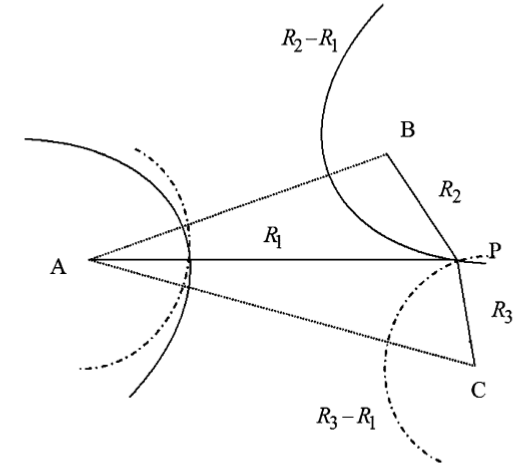
\includegraphics[width=0.5\textwidth]{images/tdoa.png}
  \caption{Positionsbestimmung mit der Differenz der Ankunftszeiten (TDOA), aus \cite{liu2007survey}. A, B und C sind die Basisstationen, die Distanzen $R_x$ werden für die Bestimmung der Position P der mobilen Einheit berechnet.}
  \label{fig:tdoa}
\end{figure}


\subsubsection{Time Difference of Arrival}
Bei TDOA wird statt der direkten Ankunftszeiten die Differenz der Ankunftszeiten gemessen. 
Dies erfordert üblicherweise Zeitsynchronität bei den Basisstationen, nicht jedoch bei der mobilen Einheit, da nur die Ankuftszeiten für die Berechnung relevant sind. Die mobile Einheit liegt dabei auf dem Schnittpunkt zweier Hyperboloiden, die jeweils zwischen den Basisstation, die TDOA gemessen haben, und einer Referenzstation aufgespannt werden. 
Die Hyperboloiden werden aufgestellt durch \\
$R_{i,j} = \sqrt{(x_i - x)^2 + (y_i - y)^2 + (z_i - z)^2} - \sqrt{(x_i - x)^2 + (y_i - y)^2 + (z_i - z)^2}$ mit $(x_i,y_i,z_i)$ als Position jeweilige Messstation, $(x_j,y_j,z_j)$ als Position der gemeinsamen Referenzstation und $(x,y,z)$ als Position der mobilen Einheit. 
Abbildung \ref{fig:tdoa} zeigt die Lösung graphisch, Drane et. al. und Torrieri beschreiben die analytische Lösung der Gleichung mit nichtlinearer Regression \cite{drane1998positioning} beziehungsweise Taylor-Entwicklung \cite{torrieri1984statistical}. 
Li et al. eliminiert zusätzlich die Forderung nach Synchronisation für mobile Einheiten, die sowohl senden als auch empfangen können \cite{li2000comparison}. 
Dabei wird ein Datenpaket an die mobile Station gesendet und von dieser mit einem \emph{Acknowledgement} beantwortet, diese Kommunikation wird von anderen Basisstationen beobachtet und die Differenz der Ankunftszeiten des Datenpakets und des \emph{Acknowledgements} als $t_{i,1}$ mit $i \in Basisstationen$ protokolliert. Zusätzlich ist $t_{i,0}$ als die Differenz zwischen dem Senden des Datenpakets und dem Empfangen an den anderen Basisstationen durch die bekannte Position aller Basisstationen ebenfalls bekannt. Damit kann die Differenz der Ankunftszeit $TDOA_{i,j} = (t_{i,0} + t_{i,1}) - (t_{j,0} + t_{j,1})$ mit $i,j \in Basisstationen$ ohne vorherige Synchronisation berechnet werden. \\


\subsubsection{Roundtrip Time of Flight}
Wird RTOF gemessen, muss die mobile Einheit sowohl senden als auch empfangen können. Dabei wird die Zeit vom Aussenden eines Paketes bis zur Ankunft der Antwort gemessen, wichtig sind hier zum einen möglichst spät/früh gesetzten Zeitstempel beim Senden/Empfangen des Signals und eine konstante Verarbeitungszeit des Kommunikationspartners. Zunächst muss dabei die Verarbeitungszeit gemessen werden, indem Basisstation und mobile Einheit auf einen Abstand von 0 Metern gebracht werden, anschließend kann die Entfernung $d = c\ *\ (t_{empfangen} - t_{gesendet} - t_{Verarbeitung})$ bestimmt werden. Die Position wird dann analog zu TOA bestimmt. Diese Messgröße kann sowohl für die Fern- als auch für die Selbstlokalisierung verwendet werden, ist aber sehr anfällig gegenüber Schwankungen in der Verarbeitungszeit, die bei Protokollen wie IEEE 802.11 häufig auftreten. \\

\subsubsection{Received Signal Strength}
RSS überprüft wie stark das empfangene Signal aus dem allgemeinen Rauschen auf der verwendeten Frequenz hervor sticht. Dafür ist es wichtig, dass immer mit der selben Leistung gesendet wird, dann kann mit einem theoretisch oder empirisch ermittelten Ausbreitungsmodell die Entfernung zwischen mobiler Einheit und Basisstation anhand des Pfadverlustes bestimmt werden. Dann ist $d = F(S_{gesendet},S_{empfangen})$ mit $F$ als Ausbreitungsmodell. Um gute Ergebnisse zu erzielen sollten jeweils möglichst gleichförmige mobile Einheiten und Basisstationen verwendet werden, denn Lui et al. konnte für IEEE 802.11 zeigen, dass unterschiedliche Hardware bei Basisstationen und mobiler Einheit erhebliche Varianz in den gemessenen RSS Werten erzeugt \cite{lui2011differences}. Zusätzliche Probleme entstehen, wenn Spezifikationen wie Bluetooth eine Anpassung der Sendeleistung vorsehen \cite{hossain2007comprehensive}, dann muss eine solche Anpassung umgangen werden. 
Bei Bluetooth geschieht das durch die Verwendung von \emph{Inquiry Paketen}, diese dienen zur Entdeckung anderer Bluetooth-fähiger Geräte und werden immer mit voller Sendeleistung gesendet um möglichst alle Geräte in Reichweite zu erreichen.
Ein weiteres Problem von RSS ist der starke Einfluss von Hindernissen und anderen  Signalen auf dem selben Frequenzband. Gerade bei der Ortung in Innenräumen wirken diese Einflüsse begrenzend auf die Genauigkeit und oft muss eine Kalibrierung durchgeführt werden um die Einflüsse von Wänden und anderen Hindernissen zu eliminieren.



\section{Grundlagen der IEEE 802.11 Spezifikation}
\label{ch:phase1:sec:grundlagen}
Die Spezifikation IEEE 802.11 beschreibt eine Form der drahtlosen Datenübertragung mittels Funkwellen \cite{ieee2012macphy}.
Sie beschreibt die physische Schicht (PHY) und den Mediumszugriff (MAC) für ein Funknetzwerk, dass mit den darüber liegenden Schichten des OSI-Modells in andere Netzwerke eingebunden werden kann.
Wird ein solches Netzwerk in ein \emph{Local Area Network} (LAN) eingebunden spricht man üblicherweise vom \emph{Wireless Local Area Network} (WLAN).
IEEE 802.11 wurde 1997 erstmals verabschiedet und wurde häufig erweitert und wird in seiner ursprünglichen Form praktisch nicht mehr angewendet, da die Datenraten zu gering sind.
Die Erweiterungen werden mit Buchstaben benannt (zum Beispiel IEEE 802.11g) und verändern etwa die verwendete Frequenz und Modulationsverfahren.\\
Zur Vermeidung von Kollisionen kommt \emph{Carrier Sense Multiple Access/Collision Avoidance} (CSMA/CA) zum Einsatz.
Bei CSMA/CA wird zunächst das Medium belauscht und gewartet bis keine Signale mehr auf dem Medium sind. 
Dann muss ein \emph{Inter Frame Spacing} (IFS) abgewartet werden, je nach Priorität ist dieses unterschiedlich lang (\emph{Short} IFS < \emph{Priority} IFS < \emph{Data} IFS < \emph{Extended} IFS), anschließend kann gesendet werden.
Tritt trotzdem eine Kollision auf, versucht der Sender es erneut mit einem längeren IFS.\\
IEEE 802.11 spezifiziert ebenfalls mehrere Operationen, die beispielsweise zur Entdeckung von Ressourcen und der Authentifizierung an einer Ressource dienen.
Einige, für diese Arbeit wichtige, Operationen werden im Folgenden beschrieben.

\subsection{Scan}
\label{ch:phase1:sec:scan}
\emph{Scan} ist eine Operation zur Entdeckung von \emph{Access Points} (APs), sie kann von einer Station (Endverbraucher, zum Beispiel Smartphone oder Laptop) passiv oder aktiv ausgeführt werden \cite{ieee2012scan}.
Bei einem passiven \emph{Scan} empfängt die \emph{Station} und filtert die von APs regelmäßig gesendeten \emph{Beacons} heraus, diese gelten dann als entdeckt.
Ein \emph{Beacon} ist ein \emph{Management Frame}, der dazu gedacht ist, technische Möglichkeiten des APs zu bewerben, zum Beispiel die möglichen Datenraten und Zeitstempel zur Synchronisierung.
Versteckte APs senden keine \emph{Beacons}. \\
Bei einem aktiven \emph{Scan} sendet die Station einen \emph{Probe Request} aus, dieser kann sowohl an alle APs (\emph{Broadcast}) als auch an einen speziellen AP adressiert sein.
Ein \emph{Probe Request} bewirbt, ähnlich wie ein \emph{Beacon}, die technischen Möglichkeiten der Station.
Der addressierte AP, beziehungsweise im Falle eines \emph{Broadcasts} alle APs, beantwortet den \emph{Probe Request} mit einer \emph{Probe Response}, in der er mitteilt, welche der beworbenen Funktionen er ebenfalls unterstützt. 
Die Station schließt den Vorgang mit einem \emph{Acknowlegement} ab. \\
Das 2,4 GHz ISM-Band wird in Europa in 13 je 10 MHz breite Kanäle aufgeteilt, da ein AP immer nur auf einem Kanal aktiv ist, müsste jeder Kanal gescannt werden.
Praktisch werden jedoch breitere Kanäle verwendet. 
IEEE 802.11g verwendet beispielsweise 20 MHz breite Kanäle, sodass effektiv nur die Kanäle 1, 5, 9 und 13 geprüft werden müssen. \\
Tabelle \ref{table:management} listet alle in der IEEE 802.11 Spezifikation gelisteten \emph{Management Frames}.
Ein \emph{Management Frame} wird durch die Typenbits markiert und durch die Bits für den Subtypen weiter unterschieden.

\begin{table}[h]
	\centering
	\caption{\emph{Management Frames} nach IEEE 802.11 \cite{ieee2012management}}
	\label{table:management}
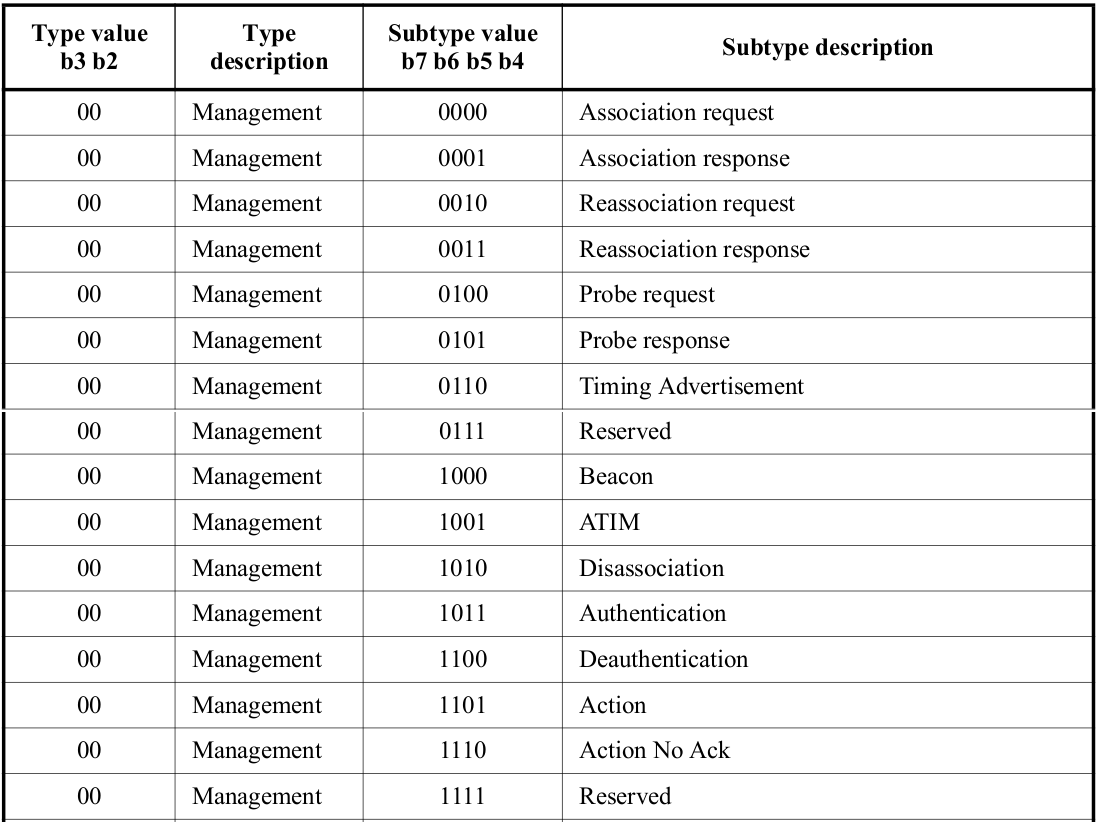
\includegraphics[width=\textwidth]{images/managementframes.png}
\end{table}

\subsection{Join}
Aus den entdeckten APs kann nun einer ausgewählt werden, um seinem Netzwerk (BSS) beizutreten \cite{ieee2012join}.
Es kann zwar geschehen, dass mehrere APs eines Netzwerks entdeckt wurden, eine Station kann jedoch zu jedem Zeitpunkt nur mit einem AP assoziert sein. \\
Um einem Netzwerk beizutreten muss sich die Station zunächst authentifizieren. 
Dieser Vorgang wird über einen \emph{Authentication Frame} (siehe Tabelle \ref{table:management}) initiiert \cite{ieee2012auth}. 
Das weitere Vorgehen hängt vom Authentifizierungsverfahren ab, zum Beispiel kann der AP einen \emph{Challenge Text} an die Station senden, der mit einem aus dem Passwort erzeugten Schlüssel verschlüsselt wird und an den AP zurück gesendet werden kann. 
Ist die Antwort korrekt, bestätigt der AP den Vorgang mit einem \emph{Acknowledgement} und eventuell zusätzlichen Informationen für eine Stromchiffre. \\
Anschließend kann die Station mit dem AP assoziiert werden \cite{ieee2012associate}. 
Sie erhält nun eine IP und der AP gibt dem Netzwerk bekannt, dass er für die Station zuständig ist. 
Dies geschieht üblicherweise über das \emph{Address Resolution Protokoll} (ARP) oder das \emph{Internet Group Management Protocol} (IGMP).\\
Ist eine Station assoziert kann sie Datenverbindungen mit anderen Teilnehmern im Netzwerk aufbauen, sie könnte beispielweise das HTTP-Protokoll nutzen, um eine Webseite anzufordern.

\subsection{Reassociation}
Eine \emph{Reassoziation} wird durchgeführt, wenn die Station keine gute Verbindung mehr zu ihrem AP hat und ein AP des selben Netzwerks verfügbar ist, der eine bessere Verbindung bietet \cite{ieee2012reassociate}.
Um diesen neuen AP zu entdecken muss zunächst ein \emph{Scan} durchgeführt werden. \\
Anschließend sendet die Station einen \emph{Reassociation Request} an den neuen AP. 
Im \emph{Reassociation Request} wird der alte AP benannt, sodass der neue AP überprüfen kann, ob die Station tatsächlich mit ihm assoziert ist, gepufferte Pakete von ihm entgegennehmen und die \emph{Assoziation} mit ihm auflösen kann.
Der Kommunikationsvorgang zwischen den APs wird auch als \emph{Handoff} bezeichnet. 
Wird dieser erfolgreich abgeschlossen antwortet der neue AP der Station mit einer \emph{Reassiciation Response}.
Abschließend wird dem Netzwerk die neue \emph{Assoziation} mittels ARP mitgeteilt.


\section{Grundlagen der Bluetooth Spezifikation}
Bluetooth beschreibt eine Form der Funkkommunikation über kurze Distanzen, die zunächst für Mobiltelefone entwickelt und dann auf weitere Geräteklassen übertragen wurde.
Ursprünglich wurde die physische Schicht (PHY) und der Mediumszugriff (MAC) in der Spezifikation IEEE 802.15.1 definiert \cite{ieee2002blue}. 
Diese wird allerdings nicht mehr vom \emph{Institute of Electrical and Electronics Engineers} (IEEE) gepflegt. \\
Bluetooth ist bereits in der Version 5.0 erschienen, da jedoch zum Zeitpunkt der Recherche für diese Arbeit kaum kompatible Geräte verfügbar waren, wird im Folgenden auf Bluetooth 4.0 Bezug genommen \cite{blue2010spec}.
Bluetooth erlaubt es nach der Entdeckung eines Kommunikationspartners und anschließendem Aufbau einer Verbindung mit ihm im 2,4 GHz ISM-Band.
Die Reichweite für die Verbindung hängt neben äußeren Hindernissen und den verwendeten Antennen auch von der jeweiligen Sendeleistung ab.
Bluetooth Geräte werden dazu in drei Klassen eingeteilt, siehe Tabelle \ref{table:blclass}.

\begin{table}[h]
  \centering
	\caption{Klasseneinteilung für Bluetooth Geräte nach Sendeleistung, aus \cite{blue2010classes}.}
	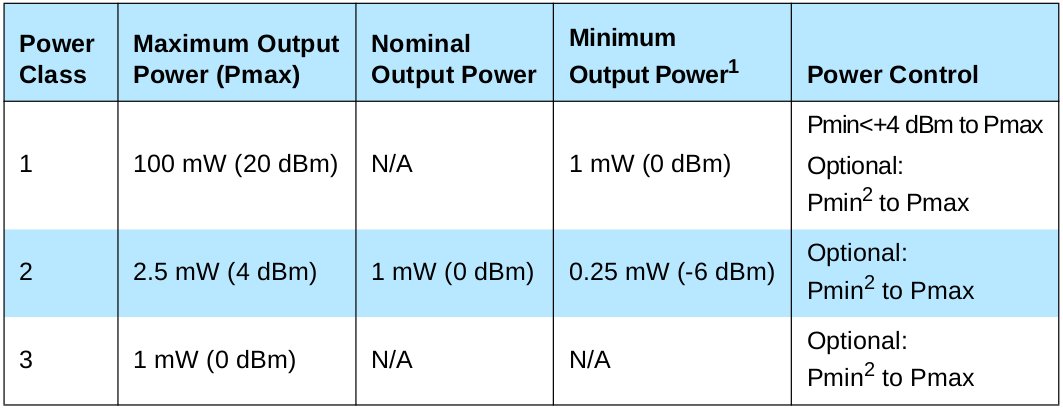
\includegraphics[width=0.9\textwidth]{images/blueclasses.png}
  \label{table:blclass}
\end{table}

Mit Bluetooth 4.0 wurde erstmals \emph{Bluetooth Low Energie} (BLE, auch Bluetooth Smart) vorgestellt.
BLE wurde für niedrigen Energieverbrauch optimiert, es verzichtet auf den Verbindungsaufbau, um den Zeitabschnitt in dem das Gerät aktiv ist zu reduzieren.
Da aber Informationen, die üblicherweise während des Verbindungsaufbaus übertragen werden, nun als \emph{Header} um das Datenpaket gepackt werden müssen, sinkt die Bruttodatenrate gegenüber Bluetooth deutlich \cite{rigado2016practical}. 
BLE eignet sich somit vor allem dann, wenn wenige oder selten Informationen ausgetauscht werden müssen.
Im Folgenden werden die, für die Lokalisation wichtigen Operationen vorgestellt.
Es handelt sich dabei jeweils um die Funktion des Entdeckens von Ressourcen mittels \emph{Inquiry Scan} für Bluetooth beziehungsweise mittels \emph{Advertising} für BLE.

\subsection{Inquiry Scan}
Eine Bluetooth-Verbindung besitzt immer einen \emph{Master} und einen \emph{Slave} \cite{blue2010inquiry}.
Da es sich beim \emph{Inquiry Scan} um eine Operation zum Entdecken von Ressourcen handelt ist, sind die Rollen noch nicht festgelegt. 
Die Spezifikation geht aber davon aus, dass der Sender der \emph{Inquiry Message} der \emph{Master} ist.
Nachdem der \emph{Master} die \emph{Inquiry Message} versendet hat antwortet der \emph{Slave} nach 625 $\mu$s mit einer \emph{Inquiry Response}. 
Soll eine erweiterte \emph{Inquiry Response} zum Einsatz kommen, wird dies in der \emph{Inquiry Response} gekennzeichnet und die erweiterte \emph{Inquiry Response} 1250 $\mu$s später gesendet.
Diese Zeiten sind den bei Bluetooth vorgesehenen Frequenzsprüngen angepasst.
Abbildung \ref{fig:inqscan} zeigt den Vorgang inklusive erweiterter \emph{Inquiry Response}.
Die Pakete sind entsprechend ihrer Inhaltsspezifikation benannt, \emph{ID} entspricht der \emph{Inquiry Message}, \emph{FHS} der \emph{Inquiry Response} und \emph{Extended Inquiry Response Packet} der erweiterten \emph{Inquiry Response}.

\begin{figure}[h]
  \centering
	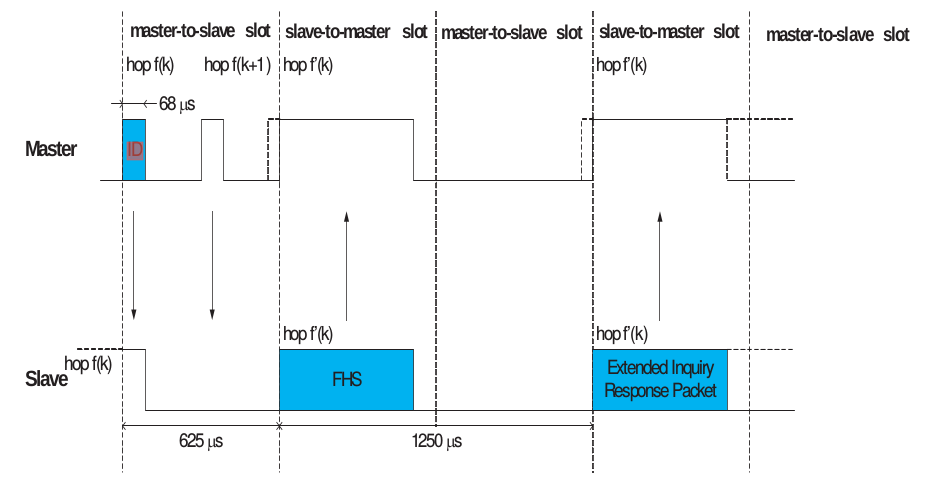
\includegraphics[width=\textwidth]{images/inqscan.png}
  \caption{\emph{Inquiry Scan} Vorgang, aus \cite{blue2010inquiry}.}
  \label{fig:inqscan}
\end{figure}

\subsection{Advertising}
Für das \emph{Advertising} stellt die Bluetooth Spezifikation drei über das Frequenzband verteilte Kanäle bereit \cite{blue2010channel}.
Auf diesen können BLE-Geräte \emph{Advertising Pakete} in einem unidirektionalen \emph{Broadcast} versenden.
\emph{Advertising} Pakete dürfen auch Nutzdaten enthalten, diese können dann von anderen, scannenden BLE-Geräten empfangen werden \cite{blue2010advertising}.
Allerdings dürfen die Nutzdaten maximal eine Länge von 31 Byte aufweisen \cite{blue2010pdu}.
Wurde zusätzlich im \emph{Advertising}-Paket markiert, dass das Gerät verbindungsfähig ist, kann ein scannendes Gerät nach empfangen des \emph{Advertising}-Paketes einen \emph{Scan Request} an das verbindungsfähige Gerät richten, um die Parameter für eine Verbindung auszuhandeln \cite{blue2010scanning}.

\section{Grundlagen von LoRa}
LoRa ist eine proprietäre Modulationstchnik und beschreibt somit eine physische Schicht.
LoRa ist für hohe Reichweite optimiert, bietet aber auch eine variable Sendeleistung, um den Energieverbrauch zu reduzieren.
LoRa beherrscht neben unterschiedlichen Frequenzen des ISM Bands, in Europa beispielsweise 433 und 868 MHz, auch eine adaptive Datenrate zwischen 0,3 und 50kbps.\\
Um den Mediumszugriff zu regeln wird die MAC-Schicht von LoRaWAN verwendet \cite{lora2015spec}.
LoRaWAN verwendet keine Kollisionsvermeidung, stattdessen dürfen Endgeräte zu jedem Zeitpunkt senden, solange sie dabei den Kanal zufällig wählen und die maximale Sendezeit beziehungsweise relative Frequenzbelegungsdauer nicht überschreiten.
Maximale Sendezeit und relative Frequenzbelegungsdauer werden dabei durch die länderspezifischen Regulierungsbehörden festgelegt.\\
LoRaWAN kann außerdem verwendet werden, wenn eine Verbindung nicht direkt zwischen zwei Kommunikationspartnern, sondern über ein \emph{Gateway} zustande kommen soll.
Dann muss diesem \emph{Gateway} zunächst beigetreten werden, danach können bestätige und unbestätigte Datenpakete über das \emph{Gateway} und ein dahinterliegendes Netzwerk ausgetauscht werden.
Tabelle \ref{table:mtype} zeigt die Nachrichtentypen von LoRaWAN.

\begin{table}[h]
  \centering
  \caption{Nachrichtentypen von LoRaWAN, aus \cite{lora2015spec}.}
	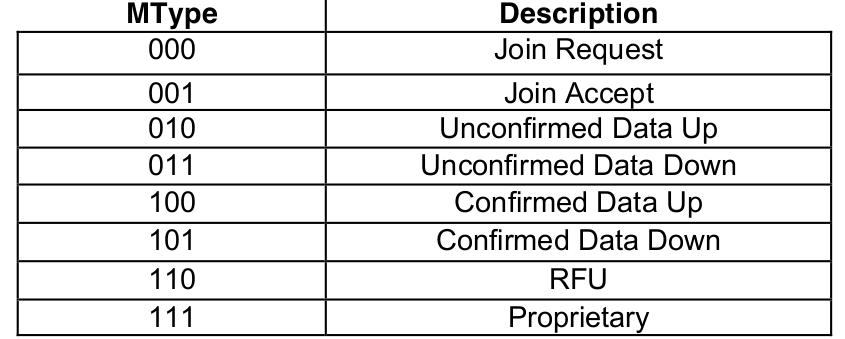
\includegraphics[width=0.8\textwidth]{images/mtype.png}
  \label{table:mtype}
\end{table}


